\documentclass[12pt]{article}

\usepackage{lscape}
\usepackage{amsmath, mathtools}
\usepackage{amsfonts}
\usepackage{amssymb}
\usepackage{graphicx}
\usepackage{colortbl}
\usepackage{xr}
\usepackage{hyperref}
\usepackage{longtable}
\usepackage{xfrac}
\usepackage{tabularx}
\usepackage{float}
\usepackage{siunitx}
\usepackage{booktabs}
\usepackage{caption}
\usepackage{pdflscape}
\usepackage{afterpage}

\usepackage[round]{natbib}

%\usepackage{refcheck}

\hypersetup{
    bookmarks=true,         % show bookmarks bar?
      colorlinks=true,       % false: boxed links; true: colored links
    linkcolor=red,          % color of internal links (change box color with linkbordercolor)
    citecolor=green,        % color of links to bibliography
    filecolor=magenta,      % color of file links
    urlcolor=cyan           % color of external links
}

%% Comments

\usepackage{color}

\newif\ifcomments\commentstrue

\ifcomments
\newcommand{\authornote}[3]{\textcolor{#1}{[#3 ---#2]}}
\newcommand{\todo}[1]{\textcolor{red}{[TODO: #1]}}
\else
\newcommand{\authornote}[3]{}
\newcommand{\todo}[1]{}
\fi

\newcommand{\wss}[1]{\authornote{blue}{SS}{#1}} 
\newcommand{\plt}[1]{\authornote{magenta}{TPLT}{#1}} %For explanation of the template
\newcommand{\an}[1]{\authornote{cyan}{Author}{#1}}


% For easy change of table widths
\newcommand{\colZwidth}{1.0\textwidth}
\newcommand{\colAwidth}{0.13\textwidth}
\newcommand{\colBwidth}{0.82\textwidth}
\newcommand{\colCwidth}{0.1\textwidth}
\newcommand{\colDwidth}{0.05\textwidth}
\newcommand{\colEwidth}{0.8\textwidth}
\newcommand{\colFwidth}{0.17\textwidth}
\newcommand{\colGwidth}{0.5\textwidth}
\newcommand{\colHwidth}{0.28\textwidth}

% Used so that cross-references have a meaningful prefix
\newcounter{defnum} %Definition Number
\newcommand{\dthedefnum}{GD\thedefnum}
\newcommand{\dref}[1]{GD\ref{#1}}
\newcounter{datadefnum} %Datadefinition Number
\newcommand{\ddthedatadefnum}{DD\thedatadefnum}
\newcommand{\ddref}[1]{DD\ref{#1}}
\newcounter{theorynum} %Theory Number
\newcommand{\tthetheorynum}{T\thetheorynum}
\newcommand{\tref}[1]{T\ref{#1}}
\newcounter{tablenum} %Table Number
\newcommand{\tbthetablenum}{T\thetablenum}
\newcommand{\tbref}[1]{TB\ref{#1}}
\newcounter{assumpnum} %Assumption Number
\newcommand{\atheassumpnum}{P\theassumpnum}
\newcommand{\aref}[1]{A\ref{#1}}

\newcounter{assumpnumS} %Scope Assumption Number
\newcommand{\atheassumpnumS}{P\theassumpnumS}
\newcommand{\aSref}[1]{AS\ref{#1}}
\newcounter{assumpnumB} %Build Assumption Number
\newcommand{\atheassumpnumB}{P\theassumpnumB}
\newcommand{\aBref}[1]{AB\ref{#1}}
\newcounter{assumpnumR} %Run-Time Assumption Number
\newcommand{\atheassumpnumR}{P\theassumpnumR}
\newcommand{\aRref}[1]{AR\ref{#1}}



\newcounter{goalnum} %Goal Number
\newcommand{\gthegoalnum}{P\thegoalnum}
\newcommand{\gsref}[1]{GS\ref{#1}}
\newcounter{instnum} %Instance Number
\newcommand{\itheinstnum}{IM\theinstnum}
\newcommand{\iref}[1]{IM\ref{#1}}
\newcounter{reqnum} %Requirement Number
\newcommand{\rthereqnum}{P\thereqnum}
\newcommand{\rref}[1]{R\ref{#1}}
\newcounter{lcnum} %Likely change number
\newcommand{\lthelcnum}{LC\thelcnum}
\newcommand{\lcref}[1]{LC\ref{#1}}

\newcommand{\famname}{Family of Lighting Models} % PUT YOUR PROGRAM NAME HERE

\usepackage{fullpage}

\begin{document}

\title{Commonality Analysis for \famname} %\plt{\famname should appear in the 
%title}} 
\author{Sasha Soraine}
\date{\today}

\maketitle

~\newpage

\pagenumbering{roman}

\section{Revision History}

\begin{tabularx}{\textwidth}{p{3cm}p{2cm}X}
\toprule {\bf Date} & {\bf Version} & {\bf Notes}\\
\midrule
October 1, 2019 & 1.0 & Original draft\\
October 17, 2019 & 1.1 & Updates in Response to GitHub Issues \\
\bottomrule
\end{tabularx}

~\newpage
	
\section{Reference Material}

This section records information for easy reference.

\subsection{Table of Units}

Throughout this document SI (Syst\`{e}me International d'Unit\'{e}s) is employed
as the unit system.  In addition to the basic units, several derived units are
used as described below.  For each unit, the symbol is given followed by a
description of the unit and the SI name.
~\newline

\renewcommand{\arraystretch}{1.2}
%\begin{table}[ht]
  \noindent \begin{tabular}{l l l} 
    \toprule		
    \textbf{symbol} & \textbf{unit} & \textbf{SI}\\
    \midrule 
    \si{\radian} & angle & radian\\
    \bottomrule
  \end{tabular}
  %	\caption{Provide a caption}
%\end{table}

%\plt{Only include the units that your CA actually uses.  If there are no units
%  for your problem, like for a general purpose library, you should still 
%include
%the heading, with the content ``not applicable'' (or similar).}

\subsection{Table of Symbols}

The table that follows summarizes the symbols used in this document along with
their units.  The choice of symbols was made to be consistent with the physics 
and calculus 
notation. The symbols are listed in alphabetical order.

\renewcommand{\arraystretch}{1.2}
%\noindent \begin{tabularx}{1.0\textwidth}{l l X}
\noindent \begin{longtable*}{l l p{12cm}} \toprule
  \textbf{symbol} & \textbf{unit} & \textbf{description}\\
  \midrule 
$\mathbb{R}$ & --- & Real numbers.  \wss{I suggest you be more
    precise and define this as the set of all real numbers.  The same comment
    applies for the set of all integers.}
  \\
  $\mathbb{Z}$ & --- & Integers.
  \\
  $\psi$ & \si[per-mode=symbol] {\radian} & Angle between the normal and halfway
  vector.
  \\
  $\theta$ & \si[per-mode=symbol] {\radian} & Angle between the viewer and the
  reflected ray.
  \\
  $\angle\theta_{i}$ & \si[per-mode=symbol] {\radian} & Angle of incidence
  between incident ray and surface normal. \wss{Why use the angle symbol for
    just these two angles?  Are they different in some way?  If not, I suggest
    you get rid of the symbol.  It seems inconsistent.}
  \\
  $\angle\theta_{r}$ & \si[per-mode=symbol] {\radian} & Angle of reflection
  between reflected ray and surface normal.
  \\
  $\theta_{1}$ & \si[per-mode=symbol] {\radian} & Angle of incidence between
  incident ray and surface normal in material 1.
  \\
  $\theta_{2}$ & \si[per-mode=symbol] {\radian} & Angle of refraction between
  refracted ray and surface normal in material 2.
  \\
  $n_{1}$ & --- & Refractive index of first material.
  \\
  $n_{2}$ & --- & Refractive index of second material.
  \\
  $n_{i}$ & --- & Refractive index of i-th material.
  \\
  $p$ & --- & Point in space or on a surface.
  \\
  $p_{0}$ & --- & Point of origin.
  \\
  $v$ & --- & Position of viewer represented as a 3D point in space.
  \\
  $P$ & --- & $n$-dimensional Vector.
  \\
  $P_{x}$ & --- & $x$ dimension of Vector $P$.
  \\
  $P_{y}$ & --- & $y$ dimension of Vector $P$.
  \\
  $P_{z}$ & --- & $z$ dimension of Vector $P$.
  \\
  $P_{i}$ & --- & $i$th dimension of Vector $P$.
  \\
  $Q$ & --- & $n$-dimensional Vector.
  \\
  $Q_{x}$ & --- & $x$ dimension of Vector $Q$.
  \\
  $Q_{y}$ & --- & $y$ dimension of Vector $Q$.
  \\
  $Q_{z}$ & --- & $z$ dimension of Vector $Q$.
  \\
  $Q_{i}$ & --- & $i$th dimension of Vector $Q$.
  \\
  $\vec{L_{i}}$ & --- & Vector form of incident ray.
  \\
  $\vec{L_{r}}$ & --- & Vector form of reflected ray.
  \\
  $\vec{v}$ & --- & Vector from point to the viewer.
  \\
  $\vec{n}$ & --- & Vector form of surface normal.
  \\
  $\vec{N}$ & --- & Unit vector of surface normal, $\vec{n}$.
  \\
  $\vec{U_{L_{i}}}$ & --- & Unit vector of incident ray, $L_{i}$.
  \\
  $\vec{h}$ & --- & Unit vector halfway between the incident ray, $L_{i}$, and
  the viewer vector, $\vec{v}$.
  \\
  $I$ & -- & Intensity (Luminance) of Light Source. \wss{Doesn't luminance have
    units?  candela per meter squared? \url{https://en.wikipedia.org/wiki/Luminance}}
  \\
  $I_{L_{i}}$ & -- & Intensity (Luminance) of Light Source $L_{i}$.
  \\
  $I_{a}$ & -- & Ambient Luminance.
  \\
  $I_{ar}$ & -- & Red Colour Ambient Luminance.
  \\
  $I_{ag}$ & -- & Green Colour Ambient Luminance.
  \\
  $I_{ab}$ & -- & Blue Colour Ambient Luminance.
  \\
  $k_{a}$ & -- & Coefficient of Ambient Reflection.
  \\
  $I_{d}$ & -- & Diffuse Luminance.
  \\
  $I_{dr}$ & -- & Red Colour Diffuse Luminance.
  \\
  $I_{dg}$ & -- & Green Colour Diffuse Luminance.
  \\
  $I_{db}$ & -- & Blue Colour Diffuse Luminance.
  \\
  $k_{d}$ & -- & Coefficient of Diffuse Reflection.
  \\
  $I_{s}$ & -- & Specular Luminance.
  \\
  $I_{sr}$ & -- & Red Colour Specular Luminance.
  \\
  $I_{sg}$ & -- & Green Colour Specular Luminance.
  \\
  $I_{sb}$ & -- & Blue Colour Specular Luminance.
  \\
  $k_{s}$ & -- & Coefficient of Specular Reflection.
  \\
  $\alpha$ & -- & Shininess Coefficient.
  \\
  $I_{T}$ & -- & Total Luminance.
  \\
  $i$ & -- & Intensity of light. \wss{What is the difference between luminance
    and intensity?  I've looked over your document and this still confuses me.
    If they are the same thing, you should just use one term.  If they are
    different, you need to clarify the difference.  I did a quick google search
    and it looks like the units of intensity are lux?}
  \\
  $i(p)$ & -- & Intensity of light at a point $p$.
  \\
  $i(p, p_{0})$ & -- & Intensity of light from point $p$ at a point $p$.
  \\
  \bottomrule
\end{longtable*}
%\plt{Use your problems actual symbols.  The si package is a good idea to use 
%for
%  units.}
%\plt{For the case of a generic numerical library, units will likely not be
%  included.  For instance, a linear ODE solver will not know the units of its
%  coefficients.}

\subsection{Abbreviations and Acronyms}

\renewcommand{\arraystretch}{1.2}
\begin{tabular}{l l} 
  \toprule		
  \textbf{symbol} & \textbf{description}\\
  \midrule 
  A & Assumption\\
  AS & Scope Time Assumption \\
  AB & Build Time Assumption \\
  AR & Run Time Assumption \\
  DD & Data Definition\\
  GD & General Definition\\
  GS & Goal Statement\\
  IM & Instance Model\\
  LC & Likely Change\\
  PS & Physical System Description\\
  R & Requirement\\
  SRS & Software Requirements Specification\\
  CA & Commonality Analysis \\
  LM & Lighting Model\\
  \famname{} & \famname{}\\
  T & Theoretical Model\\
  3D & Three Dimensional \\
  API & Application Programming Interface \\
  \bottomrule
\end{tabular}\\

%\plt{Add any other abbreviations or acronyms that you add.}
%\plt{Only include abbreviations and acronyms that are actually used.}

\newpage

\tableofcontents

~\newpage

\pagenumbering{arabic}

\section{Introduction}
An important part of computer graphics is modeling the lighting 
of objects in a virtual environment. Understanding and modeling how light 
interacts with objects of different materials is necessary to provide realistic 
lighting to virtual environments. Having an open source lighting model library 
that is reliable and robust would allow for new computer graphics programmers 
to more efficiently create scenes.

The following section provides an overview of the Commonality Analysis for a 
family of lighting models. This section explains the purpose of the document, 
scope of the family, characteristics of the intended reader, and organization 
of the document.

\subsection{Purpose of Document}
This document describes a family of lighting models to be used for computer 
graphics. This document is intended to be used as a reference to be provide the 
necessary information to verify the family of models, and implement the 
different family members. 

This document captures the problem domain, theoretical models used to address 
the problem, the commonalities and variabilities between members of the family, 
and the requirements common to those members. It serves as a starting point to 
the design and implementation of a library of lighting models, and will be 
referenced in the creation of a verification and validation plan.

\subsection{Scope of the Family} \label{sec_problem_definition}
\begin{figure}[h]
	\centering
	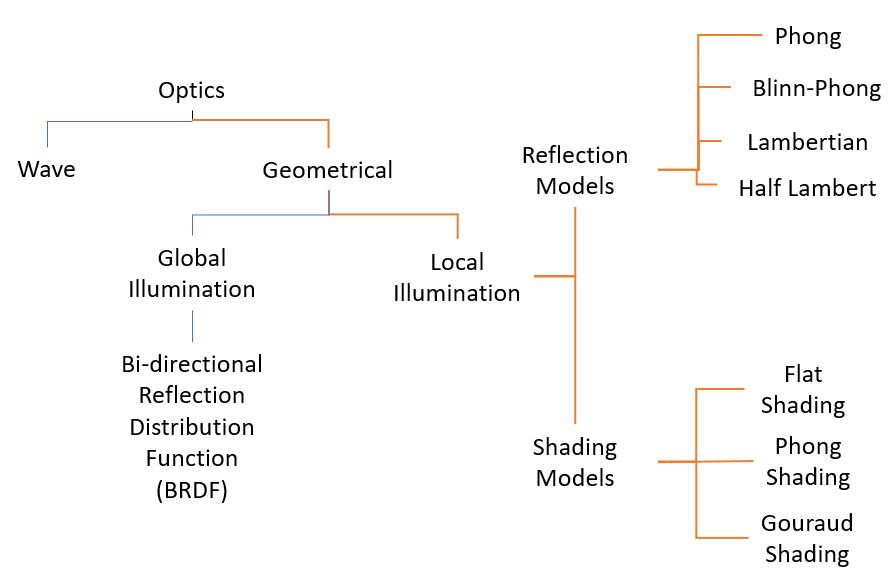
\includegraphics[scale=0.5]{./images/problem-domain-analysis}
	\caption{Problem Domain for Lighting Models of Computer Graphics.}
	\label{fig:prob-domain-analysis}
\end{figure}

The problem domain for lighting models in computer graphics is broad (Fig. 
\ref{fig:prob-domain-analysis}). To simplify this problem we invoke assumptions 
\aSref{as-geometrical_appx}, \aSref{as-illumination}, 
\aSref{as-illum_constraint}. This 
allows us to focus on the parts of the problem connected by the orange line.

The scope of the family includes geometrical optics simulation of light 
reflection for 3D material objects in a local illumination context.

\wss{Can you please explain this scope figure?  It looks like you have put some
great thinking into coming up with it, and it serves an important purpose, but
the words in the figure are not enough to explain the distinction between the
different branches.}

\subsection{Characteristics of Intended Reader}
The intended readers of this document should have understanding of Grade 12 
Physics (particularly Optics) and a undergraduate Level 2 understanding of 
Linear Algebra and Matrix operations.  

\subsection{Organization of Document}
This document is organized in accordance with the CA template for scientific 
computing software provided by Dr. Smith for CAS 741. These templates are based 
on work by \citet{Smith2006}.

\section{General System Description}
This section identifies the interfaces between the system and its environment,
describes the potential user characteristics and lists the potential system
constraints.

\subsection{Potential System Contexts}
Figure \ref{fig:system-context} shows the high level system context. The circle 
represents the system user. The box is the library of lighting models system. 
Arrows are used to show the flow of data between the system and its environment.

\begin{figure}[h]
	\centering
	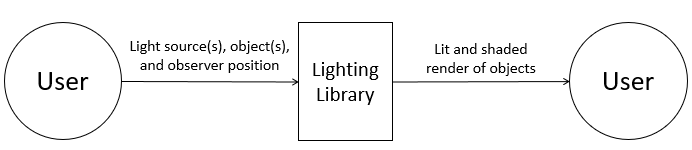
\includegraphics[scale=0.8]{./images/system-context}
	\caption{High level system context for \famname}
	\label{fig:system-context}
\end{figure}

\begin{itemize}
\item User Responsibilities:
\begin{itemize}
\item Ensure that the problem they are looking to solve matches the assumptions 
made for this family.
\item Provide information on the light source(s), object(s) in scene, and 
observer position.
\item Declare shading model to use from preset options.
\item Declare lighting model to use from present options.
\item Ensure application programming interface use complies with the user guide.
\end{itemize}
\item \famname{} Responsibilities:
\begin{itemize}
\item Calculate the reflections of all light rays coming from the light 
source(s).
\item Determine which light rays (reflected or from source) reach the observer.
\item Render a lit environment based on selected shading and lighting model.
\item Update the calculations and render in response to changes in the input 
data.
\item Detect data type mismatch, such as a string of characters instead of a
  floating point number.
\end{itemize}
\end{itemize}

\subsection{Potential User Characteristics} \label{SecUserCharacteristics}

The end user of \famname{} should have an Computer Science/Software Engineering 
Undergraduate Level 3 understanding of Computer Graphics (such as through 
completing the SFWR ENG/CS 3GC3) and moderate experience with programming.

\subsection{Potential System Constraints}
There are no system constraints.

%\plt{You may not have any system constraints.}
%
%\plt{If you need to make design decisions for your family, these decisions will
%  be made here as constraints.  For instance, if all inputs will have to use 
%the
%same file format, this would be a constraint that would be included here.}
%
%\plt{You should generally limit the number of constraints, to keep the CA
%  abstract.}

\section{Commonalities}
This section presents a high-level view of the problem. It captures terminology 
and definitions relevant to the problem, theoretical models that are common to 
all members of the family, goal statements of the family, data definitions that 
will be used to solve these problems, as well as commonalities in inputs, 
calculations, and outputs.

This section also provides a background overview which explains the motivation 
for this work.

\subsection{Background Overview} \label{Sec_Background}
Computer graphics and the techniques developed therein have become extremely 
useful in a variety of fields. Animation, games and media all rely on computer 
graphics to render semi-realistic images for their applications. As we move 
into an era of virtual and augmented reality we see that computer graphics has 
a place beyond the scope of entertainment. Training and rehabilitation 
simulations are extremely popular uses for computer graphics.

Modeling the interaction of light in realistic ways is difficult for computers. 
As such it becomes essential to have mostly accurate approximations of lights 
behaviours that can be used to render scenes in near real-time. On top of the 
need for efficient approximations, it's imperative to make the libraries and 
programs that handle lighting easy to use. It would create an incredibly high 
learning curve if users needed to understand all of the linear algebra and 
physics behind the approximations to mock up a scene. Existing paradigms for 
graphics coding offer APIs to try and make it more user friendly, but there is 
still a disproportionate focucs in graphics to manually fixing the scene and 
matrix manipulations. 

The broad purpose of this work is to abstract the details of lighting in 
computer graphics. We aim for end-users to specify their objects and light 
sources, and have the system render a fully lit and shaded scene. This type of 
work would be useful in teaching lighting model concepts, as it would easily 
allow for switching between different models. More concretely the exercise of 
understanding the family of lighting models would allow for future students to 
review this creation process and have a deeper understanding of lighting in 
computer graphics. Outside of academia, it would similarly be useful for 
individuals working on small scale graphics problems, like prototyping a 
simulation environment. Work like this would allow them to not worry about the 
math involved in getting the environment lit adequately, and instead to focus 
on their more abstract problem.

\subsection{Terminology and  Definitions}
This subsection provides a list of terms that are used in the subsequent
sections and their meaning, with the purpose of reducing ambiguity and making it
easier to correctly understand the requirements. Definitions are borrowed or 
synthesized from \cite{Lengyel2003,Comninos2005,shreiner2012}.

\begin{itemize}
%Physics/Abstract Problem 
\item[\label{}] \textit{Geometrical Optics}: The study of lights as rays.
\item[\label{}] \textit{Ray}: A view of light as a continuous beam, represented 
as a 
vector.
\item[\label{}] \textit{Reflection}: The redirection caused by collision of 
light rays 
with objects.
\item[\label{}] \textit{Specular reflection}: Perfect reflection of a light ray 
on a smooth/glossy surface. This is used to create highlights on objects, or 
create highly reflective objects like mirrors.
\item[\label{}] \textit{Diffuse (Lambertian) reflection}: Reflected light ray 
is scattered in random directions due to microfacets in the surface. This type 
of reflection does not depend of the position of an observer.
\item[\label{}] \textit{Refraction}: The redirection of light rays when passing 
through 
different materials.
\item[\label{}] \textit{Illumination}: Process by which amount of light 
reaching a 
surface is determined.
\item[\label{}] \textit{Shading}: methods used to determine the colour and 
intensity of 
light reflected towards viewer. 
\item[\label{}]\textit{ Lighting model}: Method used to calculate the colour of 
a point on a surface. Incorporates a reflection model and a shading model. 
\item[\label{}] \textit{Reflection model}: How light reflects off a surface. 
\item[\label{}] \textit{Shading model}: How the normal vector is calculated for 
polygons in the scene.
%------------Light sources--------------------------------------
\item[\label{}] \textit{Light source}: The origin of light rays.
\item[\label{}] \textit{Ambient light}: Light with no identifiable source or 
direction. It has equal intensity in every direction, and illuminates every 
part of an object uniformly.
\item[\label{}] \textit{Directional (or infinite) light}: Light defined only by 
direction; light travels infinitely in that single direction with constant 
intensity. 
\item[\label{}] \textit{Point light}: Light defined only by a point; light 
travels uniformly in every direction from that point, with intensity decreasing 
with inverse square of distance from source. 
\item[\label{}] \textit{Spotlight}: Light defined by a point and direction; 
light travels infinitely in a single direction from the defined source point 
with intensity decreasing with inverse square of distance from source and 
increased radius of coverage.
%----------------Objects-------------------------------------
\item[\label{}] \textit{Scene}: A collection of objects with specific material 
properties. 
\item[\label{}] \textit{Object}: Set of polygons, edges, and vertices. 
\item[\label{}] \textit{Polygon}: Closed shape (with well defined interior and 
exterior).
\item[\label{}] \textit{Normal}: A vector perpendicular to a surface, point, or 
pair of 
vectors.

\end{itemize}

\subsection{Data Definitions} \label{sec_datadef}
This section collects and defines all the data needed to build the instance
models. The dimension of each quantity is also given.

~\newline

\noindent
\begin{minipage}{\textwidth}
\renewcommand*{\arraystretch}{1.5}
\begin{tabular}{| p{\colAwidth} | p{\colBwidth}|}
\hline
\rowcolor[gray]{0.9}
Number& DD\refstepcounter{datadefnum}\thedatadefnum \label{DD_Dot_Product}\\
\hline
Label& \bf Dot Product of two n-dimensional vectors\\
\hline
Symbol &$P\bullet Q$\\
\hline
% Units& $Mt^{-3}$\\
% \hline
  SI Units & --\\
  \hline
  Equation&$P\bullet Q = \sum_{1}^{n}P_{i}Q_{i}$\\
  \hline
  Description & $P$ and $Q$ are two $n$-dimensional vectors. The dot product 
  ($P\bullet Q$) is the scalar sum of the products of each component. The dot 
  product acts a measure of the difference between the directions in which $P$ 
  and $Q$ point. $P$ and $Q$ are perpendicular when $P\bullet Q = 0$. This is 
  used in \tref{TM_Reflection} and \dref{GD_diffReflect}.
  \\
  \hline
  Sources& \cite{Lengyel2003}\\
  \hline
  Ref.\ By & \aBref{as-coordinate_system}, \aBref{as-coordinates}\\
  \hline
\end{tabular}
\end{minipage}\\

~\newline

\noindent
\begin{minipage}{\textwidth}
	\renewcommand*{\arraystretch}{1.5}
	\begin{tabular}{| p{\colAwidth} | p{\colBwidth}|}
		\hline
		\rowcolor[gray]{0.9}
		Number& DD\refstepcounter{datadefnum}\thedatadefnum 
		\label{DD_Cross_Product}\\
		\hline
		Label& \bf Cross Product of two 3-dimensional vectors\\
		\hline
		Symbol &$P\times Q$\\
		\hline
		% Units& $Mt^{-3}$\\
		% \hline
		SI Units & --\\
		\hline
		Equation&$P\times Q = \langle P_{y}Q_{z}-P_{z}Q_{y}, 
		P_{z}Q_{x}-P_{x}Q_{z}, P_{x}Q_{y}-P_{y}Q_{x} \rangle$ \wss{Do
                          you consistently use angle brackets to define vectors?
           I think it would be a good idea to include a section in the Reference
                          Material section that explains your notational conventions.}
          \\
		\hline
		Description & $P$ and $Q$ are two $3$-dimensional vectors. The cross 
		product ($P\times Q$) is the unit vector normal to both $P$ and $Q$. 
		The calculation of the cross product's direction follows the 
		\textit{right hand rule} paradigm. This is used in \tref{TM_Reflection} 
		and \dref{GD_diffReflect}.
		\\
		\hline
		Sources& \cite{Lengyel2003}\\
		\hline
		Ref.\ By & \aBref{as-coordinate_system}, \aBref{as-coordinates} \\
		\hline
	\end{tabular}
\end{minipage}\\

~\newline

\noindent
\begin{minipage}{\textwidth}
	\renewcommand*{\arraystretch}{1.5}
	\begin{tabular}{| p{\colAwidth} | p{\colBwidth}|}
		\hline
		\rowcolor[gray]{0.9}
		Number& DD\refstepcounter{datadefnum}\thedatadefnum 
		\label{DD_Intensity_ambient}\\
		\hline
		Label& \bf Ambient Luminance for a Light Source\\
		\hline
		Symbol &$I_{a}$\\
		\hline
		% Units& $Mt^{-3}$\\
		% \hline
		SI Units & -- \wss{I wrote this elsewhere, but shouldn't
                           luminance have units?}\\
		\hline
		Equation&$I_{a} = \begin{Bmatrix}
		I_{ar} \\ I_{ag} \\ I_{ab} \\
		\end{Bmatrix} = I_{L_{i}}\cdot k_{a}$\\
		\hline
		Description & $I_{L{i}}$ is the intensity of the light source - it is 
		uniform for ambient light and shouldn't rely on position. \\
		& $k_{a}$ is the coefficient of ambient reflection.  \wss{Please
          define all of the symbols in all of your DDs, GDs, etc.}\\
		\hline
		Sources& \cite{shreiner2012}\\
		\hline
		Ref.\ By & \iref{IM_LamDiffuse}, \iref{IM_HalfLam}, \iref{IM_Phong}, 
		\iref{IM_Blinn_Phong}\\
		\hline
	\end{tabular}
\end{minipage}\\


~\newline

\noindent
\begin{minipage}{\textwidth}
	\renewcommand*{\arraystretch}{1.5}
	\begin{tabular}{| p{\colAwidth} | p{\colBwidth}|}
		\hline
		\rowcolor[gray]{0.9}
		Number& DD\refstepcounter{datadefnum}\thedatadefnum 
		\label{DD_Intensity_diffuse}\\
		\hline
		Label& \bf Diffuse Luminance for a Light Source\\
		\hline
		Symbol &$I_{d}$\\
		\hline
		% Units& $Mt^{-3}$\\
		% \hline
		SI Units & --\\
		\hline
		Equation&$I_{d} = \begin{Bmatrix}
		I_{dr} \\ I_{dg} \\ I_{db} \\
		\end{Bmatrix} = k_{d}\cdot I_{L_{i}}(p)(\vec{U_{i}}\bullet \vec{N}) 
		L_{d}$\\
		\hline
		Description & $p$ is the point where $\vec{L_{i}}$ hits the surface.
		\\
		& $I_{L_{i}}(p)$ is the intensity of $L_{i}$ at point $p$. \\
		& $k_{d}$ is the coefficient of diffuse reflection. \\
		& $\vec{U_{i}}$ is the unit vector of $L_{i}$. \\
		& $\vec{N}$ is the unit vector surface normal. \\
		\hline
		Sources& \cite{shreiner2012}\\
		\hline
		Ref.\ By & \iref{IM_LamDiffuse}, \iref{IM_HalfLam}, \iref{IM_Phong}, 
		\iref{IM_Blinn_Phong} \\
		\hline
	\end{tabular}
\end{minipage}\\

~\newline

\noindent
\begin{minipage}{\textwidth}
	\renewcommand*{\arraystretch}{1.5}
	\begin{tabular}{| p{\colAwidth} | p{\colBwidth}|}
		\hline
		\rowcolor[gray]{0.9}
		Number& DD\refstepcounter{datadefnum}\thedatadefnum 
		\label{DD_Intensity_specular}\\
		\hline
		Label& \bf Specular Luminance for a Light Source\\
		\hline
		Symbol &$I_{s}$\\
		\hline
		% Units& $Mt^{-3}$\\
		% \hline
		SI Units & --\\
		\hline
		Equation&$I_{s} = \begin{Bmatrix}
		I_{sr} \\ I_{sg} \\ I_{sb} \\
		\end{Bmatrix} = k_{s}L_{s}\max((\vec{U_{r}}\bullet \vec{v})^\alpha, 0)
		$ \\
		\hline
		Description & $p_{0}$ is the position of the light source in Cartesian 
		Coordinates.
		\\
		& $\vec{U_{r}}$ is the unit vector of the reflected ray.\\
		& $\vec{v}$ is the vector to the viewer.\\
		& $k_{s}$ is the specular coefficient of the material.\\
		& $\alpha$ is the shininess coefficient to determine the size of the 
		specular highlight.\\
		& 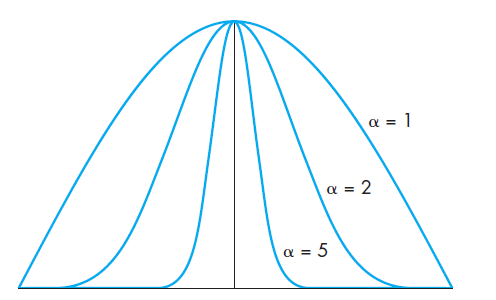
\includegraphics[]{./images/shininess-coefficient}\\
		\hline
		Sources& \cite{shreiner2012}\\
		\hline
		Ref.\ By & \iref{IM_Phong}, \iref{IM_Blinn_Phong}\\
		\hline
	\end{tabular}
\end{minipage}\\

~\newline

\noindent
\begin{minipage}{\textwidth}
	\renewcommand*{\arraystretch}{1.5}
	\begin{tabular}{| p{\colAwidth} | p{\colBwidth}|}
		\hline
		\rowcolor[gray]{0.9}
		Number& DD\refstepcounter{datadefnum}\thedatadefnum 
		\label{DD_Intensity_Total}\\
		\hline
		Label& \bf Total Luminance for a Light Source\\
		\hline
		Symbol &$I_{T}$\\
		\hline
		% Units& $Mt^{-3}$\\
		% \hline
		SI Units & --\\
		\hline
		Equation&$I_{T} = I_{a} + I_{d} + I_{s}$ \\
		\hline
		Description & Total luminance is the combination of ambient, diffuse, 
		and specular luminance.
		\\
		\hline
		Sources& \cite{shreiner2012}\\
		\hline
		Ref.\ By & \iref{IM_Phong} \\
		\hline
	\end{tabular}
\end{minipage}\\

~\newline

\noindent
\begin{minipage}{\textwidth}
	\renewcommand*{\arraystretch}{1.5}
	\begin{tabular}{| p{\colAwidth} | p{\colBwidth}|}
		\hline
		\rowcolor[gray]{0.9}
		Number& DD\refstepcounter{datadefnum}\thedatadefnum 
		\label{DD_Intensity_PointSource_Distance}\\
		\hline
		Label& \bf Intensity of illumination at point $p$ from a point source, 
		$p_{0}$\\
		\hline
		Symbol &$i(p, p_{0})$\\
		\hline
		% Units& $Mt^{-3}$\\
		% \hline
		SI Units & --\\
		\hline
		Equation&$i(p, p_{0}) = \frac{1}{|p-p_{0}|^2} I(p_{0})$\\
		\hline
		Description & Calculates the intensity of light at point $p$ from a 
		light source at position $p_{0}$ in Cartesian Coordinates.
		\\
		\hline
		Sources& \cite{Lengyel2003}\\
		\hline
		Ref.\ By & \aBref{as-coordinate_system}, \aBref{as-coordinates} \\
		\hline
	\end{tabular}
\end{minipage}\\

~\newline

\noindent
\begin{minipage}{\textwidth}
	\renewcommand*{\arraystretch}{1.5}
	\begin{tabular}{| p{\colAwidth} | p{\colBwidth}|}
		\hline
		\rowcolor[gray]{0.9}
		Number& DD\refstepcounter{datadefnum}\thedatadefnum 
		\label{DD_Flat_Shading}\\
		\hline
		Label& \bf Calculation of Normals for Flat Shading\\
		\hline
		Symbol &$\vec{n}$\\
		\hline
		% Units& $Mt^{-3}$\\
		% \hline
		SI Units & --\\
		\hline
		Equation&$\vec{n} = \frac{\vec{P} \times \vec{Q}}{|\vec{P} \times 
		\vec{Q}|}$\\
		\hline
		Description & Flat shading calculates the surface normal of a polygon 
		in a mesh. Given two non-parallel vectors tangent to the surface of the 
		polygon, $\vec{P}$ and $\vec{Q}$,the normal ($\vec{n}$) is 
		the normalized cross-product of $\vec{P}$ and $\vec{Q}$ \\
		\hline
		Sources& \cite{shreiner2012}\\
		\hline
		Ref.\ By & \aBref{as-coordinate_system}, \aBref{as-coordinates} \\
		\hline
	\end{tabular}
\end{minipage}\\

~\newline

\noindent
\begin{minipage}{\textwidth}
	\renewcommand*{\arraystretch}{1.5}
	\begin{tabular}{| p{\colAwidth} | p{\colBwidth}|}
		\hline
		\rowcolor[gray]{0.9}
		Number& DD\refstepcounter{datadefnum}\thedatadefnum 
		\label{DD_Gouraud_Shading}\\
		\hline
		Label& \bf Calculation of Normals for Gouraud Shading\\
		\hline
		Symbol &$\vec{n_{v}}$\\
		\hline
		% Units& $Mt^{-3}$\\
		% \hline
		SI Units & --\\
		\hline
		Equation&$\vec{n_{v}} = 
		\frac{\sum_{i=1}^{t_{v}}n_{i}}{|\sum_{i=1}^{t_{v}}n_{i}|}$\\
		\hline
		Description & Gouraud shading calculates the normal at the vertices of 
		a polygon in a mesh. Given a vertex, $v$,the normal ($\vec{n_{v}}$) is 
		the normalized average of the surface normals ($\vec{n_{i}}$) for all 
		polygons that share that vertex. $t_{v}$ is the number of polygons that 
		share the vertex $v$.\\
		& 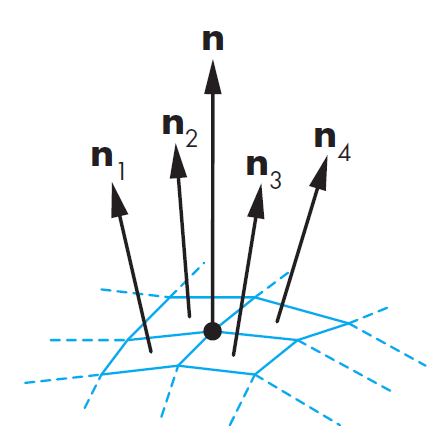
\includegraphics[]{./images/gouraud-shading-interpolation}\\
		\hline
		Sources& \cite{shreiner2012}\\
		\hline
		Ref.\ By & \aBref{as-coordinate_system}, \aBref{as-coordinates}\\
		\hline
	\end{tabular}
\end{minipage}\\

~\newline

\wss{You talk about surfaces, and polygons, but I don't see how you actually
  represent an object.  Searching through again, I see that objects have a set
  of possible shapes, but I don't see the connection between the shapes and
  polygons.  The shapes are mathematical defined, especially something like a
  sphere or a cube.  I think you need to say somewhere that you approximate the
  shape with a mesh of polygons.  You might want to look at the commonality
  analysis of mesh generators that I wrote with a student years ago.  It should
  be in our cas741 repo under CAS 04-10-SS.pdf.}

\noindent
\begin{minipage}{\textwidth}
	\renewcommand*{\arraystretch}{1.5}
	\begin{tabular}{| p{\colAwidth} | p{\colBwidth}|}
		\hline
		\rowcolor[gray]{0.9}
		Number& DD\refstepcounter{datadefnum}\thedatadefnum 
		\label{DD_Phong_Shading}\\
		\hline
		Label& \bf Calculation of Normals for Phong Shading\\
		\hline
		Symbol &$\vec{n_{v}}$\\
		\hline
		% Units& $Mt^{-3}$\\
		% \hline
		SI Units & --\\
		\hline
		Equation& \\
		\hline
		Description & Phong shading linearly interpolates normals across each 
		the surface of the polygon from the vertex normals. Surface normals are 
		then normalized per pixel.\\
		& 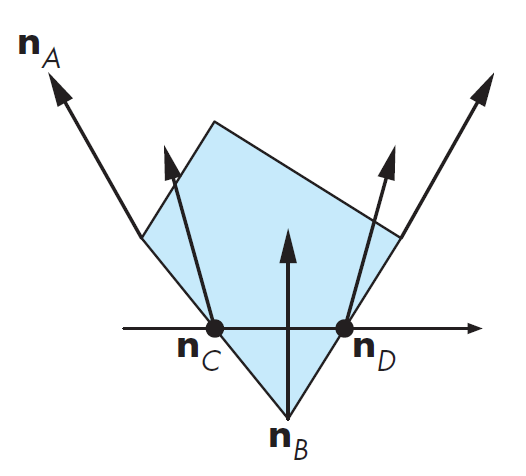
\includegraphics[]{./images/phong-shading-interpolation} \\
		\hline
		Sources& \cite{shreiner2012}\\
		\hline
		Ref.\ By & \aBref{as-coordinate_system}, \aBref{as-coordinates} \\
		\hline
	\end{tabular}
\end{minipage}\\


\subsection{Goal Statements}

\noindent Given some light source(s), some object(s) and their respective 
material properties, and an observer the goal statements are:

\begin{itemize}

\item[GS\refstepcounter{goalnum}\thegoalnum \label{gs-display}:] 
Render a fully lit and shaded scene of the objects based on the observer 
location.
%\plt{One
%    sentence description of the goal.  There may be more than one.  Each Goal
%    should have a meaningful label.}

\wss{I like this goal statement.  However, I feel like the rest of the document
  doesn't completely refine it.  I feel like there should be an instance model
  that takes the refined version of these inputs and outputs a refined version
  of the output.}

\end{itemize}

\subsection{Theoretical Models} \label{sec_theoretical}

This section focuses on the general equations and laws that \famname{} is based
on.  %\plt{Modify the examples below for your problem, and add additional models
%  as appropriate.}

~\newline

\noindent
\begin{minipage}{\textwidth}
\renewcommand*{\arraystretch}{1.5}
\begin{tabular}{| p{\colAwidth} | p{\colBwidth}|}
  \hline
  \rowcolor[gray]{0.9}
  Number& T\refstepcounter{theorynum}\thetheorynum \label{TM_Reflection}\\
  \hline
  Label&\bf Law of Reflection\\
  \hline
  Equation&   $\angle\theta_{i} = \angle\theta_{r}$ or 
  $\vec{L_{i}}\bullet\vec{N} = 
  \vec{L_{r}}\bullet\vec{N}$\\
  \hline
  Description & 
                When a ray of light reflects off a surface, the angle of 
                incident is equal to the angle of reflection. This can also be 
                written as the dot product of the incident ray and the normal 
                is equal to the dot product of the reflected ray and the 
                normal.
		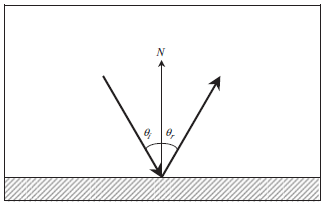
\includegraphics[scale=1]{./images/specular-reflection}  
		\\              
                                
  \hline
  Source & \cite{Comninos2005}\\
  \hline
  Ref.\ By & \dref{GD_diffReflect}\\
  \hline
\end{tabular}
\end{minipage}\\

~\newline

%\plt{In a CA, the TMs often do not need to be refined.  However, this is not a
%  rule.  In some cases, it may make sense to introduce an IM, or possibly even 
%a
%  GD in between the TM and the IM.}

\subsubsection{General Definitions}\label{sec_gendef}

%\plt{General Definitions (GDs) are a refinement of one or more TMs, and/or of
%	other GDs.  The GDs are less abstract than the TMs.  Generally the reduction
%	in abstraction is possible through invoking (using/referencing) Assumptions.
%	For instance, the TM could be Newton's Law of Cooling stated abstracting.  
%	The GD could take the general law and apply it to get a 1D equation.}

This section collects the laws and equations that will be used in building the
instance models.

%\plt{Some projects may not have any content for this section, but the section
%	heading should be kept.}  \plt{Modify the examples below for your problem, 
%	and
%	add additional definitions as appropriate.}

~\newline

\noindent
\begin{minipage}{\textwidth}
	\renewcommand*{\arraystretch}{1.5}
	\begin{tabular}{| p{\colAwidth} | p{\colBwidth}|}
		\hline
		\rowcolor[gray]{0.9}
		Number& GD\refstepcounter{defnum}\thedefnum \label{GD_diffReflect}\\
		\hline
		Label &\bf Diffuse Reflection \\
		\hline
		% Units&$MLt^{-3}T^0$\\
		% \hline
		SI Units& - \\
		\hline
		Equation& $ \angle\theta_{i} = \angle\theta_{r}$ or 
		$\vec{L_{i}}\bullet\vec{N} = 
		\vec{L_{r}}\bullet\vec{N}$  \\
		\hline
		Description &
		Law of Reflection applied to rough surfaces.
		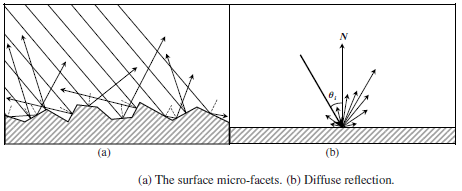
\includegraphics[scale=1]{./images/diffuse-reflection}
		\\
		\hline
		Source & \cite{Comninos2005} \\
		\hline
		Ref.\ By & \ddref{DD_Dot_Product}\\
		\hline
	\end{tabular}
\end{minipage}\\

\section{Variabilities}
The follow section outlines variabilities between family members. Section 
\ref{sec_Assumptions} covers the assumptions made to simplify/realise the 
problem. Section \ref{sec_Calculation} captures variabilities in the 
implementation.

Before tackling those sections, we summarize here variabilities in the problem.

\subsection{Assumptions} \label{sec_Assumptions}
This section outlines the various assumptions made in defining this problem.  
These are divided based on their binding time. All assumptions are used to 
support the \ref{gs-display}

\begin{itemize}
	\item \textbf{Scope Time Bindings}:
	\begin{itemize}
		\item[AS\refstepcounter{assumpnumS}\theassumpnumS\label{as-geometrical_appx}:]
		Light will be defined by Geometrical Optics principles (ray-based).
		\item[AS\refstepcounter{assumpnumS}\theassumpnumS\label{as-illumination}:]
		Lighting will be handled at the local illumination level.
		\item[AS\refstepcounter{assumpnumS}\theassumpnumS\label{as-loc-vs-global}:]
		Objects will not cast shadows on each other.		
		\item[AS\refstepcounter{assumpnumS}\theassumpnumS\label{as-illum_constraint}:]
		Objects will not reflect light at each other.
		\item[AS\refstepcounter{assumpnumS}\theassumpnumS\label{as-emission_constraint}:]
		Objects will not emit light.		
	\end{itemize}
	\item \textbf{Build Time Bindings}:
	\begin{itemize}
		\item[AB\refstepcounter{assumpnumB}\theassumpnumB\label{as-coordinate_system}:]
		 The virtual environment will be described by a 3D Caretsian Coordinate 
		System using right-hand rules.
		\item[AB\refstepcounter{assumpnumB}\theassumpnumB\label{as-coordinates}:]
		Positions of light source(s), object(s), and the observer will be 
		defined on a 3D Cartesian Coordinate System.
		\item[AB\refstepcounter{assumpnumB}\theassumpnumB\label{as-obsv_total}:]
		There will only be a single observer in a scene.				
		\item[AB\refstepcounter{assumpnumB}\theassumpnumB\label{as-object_representation}:]
		Objects will be represented by a geometric mesh of triangles.
		\item[AB\refstepcounter{assumpnumB}\theassumpnumB\label{as-object_representation2}:]
		Object meshes will be closed and convex (there is a well defined 
		interior and exterior).				
		\item[AB\refstepcounter{assumpnumB}\theassumpnumB\label{as-object_refraction}:]
		All objects are opaque; light will not experience refraction with any 
		object. 
	\end{itemize}
	\item \textbf{Run-Time Bindings}: These were captured as inputs to the 
	system.
\end{itemize}

\wss{The scope time bindings make sense, but I am not sure how to interpret the
  building time bindings.  Since they are build time, I'm assuming that whether
  they apply or not is a build time decision.  Is this correct?  If so, it feels
like if the assumptions do not apply another assumption will have to take its
place, but I don't know what that assumption is.  For instance, if the object is
not represented by a mesh of triangles, what is it represented by?}

\wss{I see the connection between the objects and their representation by
  polygons is given here.  I mentioned this in an earlier comment, but I had
  missed this mention.  However, I think you still need more information.  What
  does it mean to represent an object by a mesh?  In the mesh generator CA that
  I mentioned in an earlier comment a mesh is defined as covering up of a
  domain, with several rules.  You might want to look at that definition.}

\wss{Is the dimension of the problem a variability, or are lighting problems in
  3D?}

\subsection{Calculation} \label{sec_Calculation}
This section outlines variabilities in design details, capturing variabilities 
in: input, calculations, algorithms, and data structures.

Input variabilities: 
\begin{table}[H]
	\centering
	\begin{tabular}{|p{5cm}|p{6cm}|p{4cm}|p{1cm}|}
		\hline
		\textbf{Variability} & \textbf{Parameter of Variation} & 
		\textbf{Constraints} &  \textbf{Related} \\
		\hline
		Model room size $\langle h,w,d \rangle$ & Set of $\mathbb{R}$
                                                          \wss{The types don't
                                                          match.  You have a
                                                          vector? tuple? of 3
                                                          real numbers for the
                                                          size of the room, but
                                                          the parameters of
                                                          variation is a set of
                                                          real numbers.} & -- & 
		\aBref{as-coordinates}\\
		\hline
		Allowed values for position of light source $\langle x,y,z \rangle$ & 
		Set of 
		$\mathbb{R}$ \wss{The same comment as above applies.} & Must be in room boundaries. Light source cannot be 
		inside of an object. Light source cannot be on top of another light 
		source or on top of the observer. & \aBref{as-coordinates}\\
		\hline
		Allowed values for position of object(s) $\langle x,y,z \rangle$ & Set 
		of $\mathbb{R}$ & Object(s) must be in room boundaries. Objects must 
		not overlap with each other or a light source & 
		\aBref{as-coordinates}\\
		\hline
		Allowed values for position of observer $[x,y,z]$ & Set of $\mathbb{R}$ 
		& Observer must be in room boundaries. & \aBref{as-coordinates}\\
		\hline				
		Allowed values for colour of light $\langle r,g,b \rangle$ & Set of 
		$\mathbb{Z}$ 
		& 0 - 256 & --\\
		\hline
		Allowed values for colour of object $\langle r,g,b \rangle$ & Set of 
		$\mathbb{Z}$ 
		& 0 - 256 \wss{Why not just define a type for the integers
                  between 0 and 256?  A similar comment applies elsewhere in
                  this table.} & --\\
		\hline
		Reflection coefficient of material	& $k_{a} \in \mathbb{R}$ & $0 \le 
		k_{a} \le 1$ & -- \\
		\hline		
		Specular coefficient of material & $k_{s} \in \mathbb{R}$ & $0 \le 
		k_{s} \le 1$ & -- \\
		\hline
		Diffuse coefficient of material	& $k_{d} \in \mathbb{R}$ & & -- \\
		\hline
		Shininess coefficient of material	& $\alpha \in \mathbb{R}$ & -- & -- 
		\\
		\hline				
		Type of light source & Set of $\{Point, Spot, Directional, Ambient\}$ & 
		-- 
		& --\\
		\hline
		Type of object(s) & Set of $\{Sphere, Cube, Torus, Teapot\}$ & -- & 
		--\\
		\hline
		Type of shading & Set of $\{Flat, Gouraud, Phong\}$ & -- & 
		--\\
		\hline
		Number of object(s) & Set of $\mathbb{R}$ & -- & 
		--\\
		\hline
		Number of light(s) & Set of $\mathbb{R}$ & -- & 
		--\\
		\hline
		Number of observer(s) & Set of $\mathbb{R}$ & No. observers = 1 & 
		--\\
		\hline
		Input method & Single file with light, object and other data; multiple 
		files (one for lights and one for objects) & -- & 
		--\\
		\hline								
	\end{tabular}
	\caption{Parameters of Variation for Input.}
	\label{tbl:Input_Variations}
\end{table}

Calculation variabilities:
\begin{table}[h]
	\centering
	\begin{tabular}{|p{5cm}|p{5cm}|p{2cm}|p{2cm}|}
		\hline
		\textbf{Variability} & \textbf{Parameters of Variation} & Constraints & 
		\textbf{Ref.}\\
		\hline
		Interpolation of normals for shading & Set of 
		$\{$\ddref{DD_Flat_Shading}, \ddref{DD_Gouraud_Shading}, 
		\ddref{DD_Phong_Shading}$\}$ & -- & \aSref{as-coordinate_system} \\
		\hline		
	\end{tabular}
	\caption{Parameters of Variation in Calculations.}
\end{table}

\subsubsection{Instance Models} \label{sec_instance}    

This section transforms the problem defined in 
Section~\ref{sec_problem_definition} into one which is expressed in 
mathematical terms. It uses concrete symbols defined in 
Section~\ref{sec_datadef} to replace the abstract symbols in the models 
identified in Sections~\ref{sec_theoretical} and~\ref{sec_gendef}.

~\newline

%Instance Model 1

\noindent
\begin{minipage}{\textwidth}
	\renewcommand*{\arraystretch}{1.5}
	\begin{tabular}{| p{\colAwidth} | p{\colBwidth}|}
		\hline
		\rowcolor[gray]{0.9}
		Number& IM\refstepcounter{instnum}\theinstnum \label{IM_LamDiffuse}\\
		\hline
		Label& \bf Lambertian (Diffuse) Reflection Model\\
		\hline
		Input& $\vec{L_{i}}$, $p_{0}$, object\\
		& \\
		\hline
		Output& $\vec{L_{r}}$  \\
		&  $I_{d}$\\
		\hline
		Description & $L_{i}$ is the vector representation of the incident 
		ray.\\
		& $U_{i}$ is the unit vector of $L_{i}$.\\
		& $\vec{N}$ is the surface normal unit vector. \\
		& $p_{0}$ is the point the incident ray intercepts the surface of an 
		object. \\
		& $k_{d}$  is the coefficient of diffuse reflection.\\
		& $I_{L_{i}p_{0}}$ is the intensity of the light at point $P$\\
		& This IM is a concrete refinement on \dref{GD_diffReflect} by modeling 
		the interactions of a single light ray at a single point.\\
		\hline
		Sources& \cite{Comninos2005,Lengyel2003,shreiner2012} \\
		\hline
		Ref.\ By & \iref{IM_HalfLam}\\
		\hline
	\end{tabular}
\end{minipage}\\

\wss{As Peter pointed out on GitHub, the instance models are incomplete.  Think
  about refining the inputs and outputs.  Including type information with the
  inputs could help.  In particular, object is still vague at this point, and
  you need it to be precise before you can do a calculation.  How the outputs
  are calculated is also needed.}  ~\newline

\noindent
\begin{minipage}{\textwidth}
	\renewcommand*{\arraystretch}{1.5}
	\begin{tabular}{| p{\colAwidth} | p{\colBwidth}|}
		\hline
		\rowcolor[gray]{0.9}
		Number& IM\refstepcounter{instnum}\theinstnum \label{IM_HalfLam}\\
		\hline
		Label& \bf Half Lambert (Diffuse) Reflection Model\\
		\hline
		Input& $\vec{L_{i}}$, $p_{0}$, object\\
		\hline
		Output&  $\vec{L_{r}}$  \\
		&  $I_{d}$\\
		\hline
		Description & $L_{i}$ is the vector representation of the incident 
		ray.\\
		& $U_{i}$ is the unit vector of $L_{i}$.\\
		& $\vec{N}$ is the surface normal unit vector. \\
		& $p_{0}$ is the point the incident ray intercepts the surface of an 
		object. \\
		& $k_{d}$  is the coefficient of diffuse reflection.\\
		& $I_{L_{i}p_{0}}$ is the intensity of the light at point $P$\\
		& This IM is a concrete refinement on \iref{IM_LamDiffuse} by halving 
		the dot product of the $\vec{U_{i}}$ and $\vec{N}$ to create a softer 
		shading.\\
		\\
		\hline
		Sources& \cite{Comninos2005,Lengyel2003,shreiner2012} \\
		\hline
		Ref.\ By & \\
		\hline
	\end{tabular}
\end{minipage}\\

~\newline

\noindent
\begin{minipage}{\textwidth}
	\renewcommand*{\arraystretch}{1.5}
	\begin{tabular}{| p{\colAwidth} | p{\colBwidth}|}
		\hline
		\rowcolor[gray]{0.9}
		Number& IM\refstepcounter{instnum}\theinstnum \label{IM_Phong}\\
		\hline
		Label& \bf Phong Reflection Model\\
		\hline
		Input& $\vec{n}$, $p$, $v$, $\vec{L_{i}}$, $I_{a_{L_{i}}}$, 
		$I_{d_{L_{i}}}$, $I_{s_{L_{i}}}$\\
		& \\
		\hline
		Output& $\vec{v}$, $\vec{L_{r}}$, $I_{a_{L_{r}}}$, $I_{d_{L_{r}}}$, 
		$I_{s_{L_{r}}}$ \\
		& \\
		\hline
		Description& $p$ is a point on the polygon surface.\\
		& $v$ is the position of the viewer.\\
		& $\vec{L_{i}}$ is the incident ray hitting point $p$.\\
		& $\vec{n}$ is the surface normal at point $p$.\\
		& $I_{a_{L_{i}}}$ is the ambient intensity of the light described by 
		$L_{i}$.\\
		& $I_{d_{L_{i}}}$ is the diffuse intensity of the light described by 
		$L_{i}$. \\
		& $I_{s_{L_{i}}}$ is the specular intensity of the light described by 
		$L_{i}$. \\
		& $\vec{v}$ is the vector in the direction of the viewer from $p$.\\
		& $\vec{L_{r}}$ is the perfectly reflected ray.\\
		& $I_{a_{L_{r}}}$ is the ambient intensity of the light described by 
		$L_{r}$.\\
		& $I_{d_{L_{r}}}$ is the diffuse intensity of the light described by 
		$L_{r}$. \\
		& $I_{s_{L_{r}}}$ is the specular intensity of the light described by 
		$L_{r}$. \\
				
		& 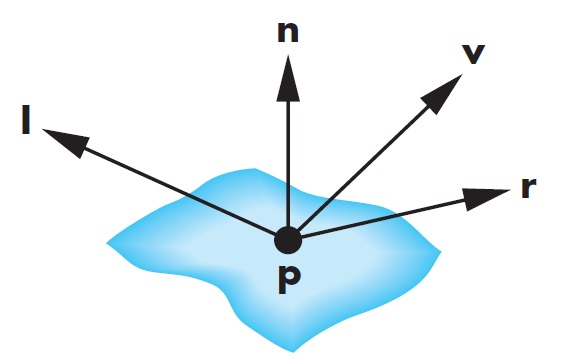
\includegraphics[scale=0.4]{./images/phong-reflection-model-vectors}\\
		\hline
		Sources& \cite{Comninos2005,Lengyel2003,shreiner2012} \\
		\hline
		Ref.\ By & \iref{IM_Blinn_Phong}\\
		\hline
	\end{tabular}
\end{minipage}\\

~\newline

\noindent
\begin{minipage}{\textwidth}
	\renewcommand*{\arraystretch}{1.5}
	\begin{tabular}{| p{\colAwidth} | p{\colBwidth}|}
		\hline
		\rowcolor[gray]{0.9}
		Number& IM\refstepcounter{instnum}\theinstnum \label{IM_Blinn_Phong}\\
		\hline
		Label& \bf Blinn-Phong Reflection Model\\
		\hline
		Input& $\vec{n}$, $p$, $v$, $\vec{L_{i}}$, $I_{a_{L_{i}}}$, 
		$I_{d_{L_{i}}}$, $I_{s_{L_{i}}}$\\
		\hline
		Output& $\vec{v}$, $\vec{h}$, $I_{a_{h}}$, $I_{d_{h}}$, 
		$I_{s_{L_{r}}}$ \\		
		\hline
		Description& $p$ is a point on the polygon surface.\\
		& $v$ is the position of the viewer.\\
		& $\vec{L_{i}}$ is the incident ray hitting point $p$.\\
		& $\vec{n}$ is the surface normal at point $p$.\\
		& $I_{a_{L_{i}}}$ is the ambient intensity of the light described by 
		$L_{i}$.\\
		& $I_{d_{L_{i}}}$ is the diffuse intensity of the light described by 
		$L_{i}$. \\
		& $I_{s_{L_{i}}}$ is the specular intensity of the light described by 
		$L_{i}$. \\
		& $\vec{v}$ is the vector in the direction of the viewer from $p$.\\
		& $\vec{L_{r}}$ is the perfectly reflected ray.\\
		& $I_{a_{L_{r}}}$ is the ambient intensity of the light described by 
		$L_{r}$.\\
		& $I_{d_{L_{r}}}$ is the diffuse intensity of the light described by 
		$L_{r}$. \\
		& $I_{s_{L_{r}}}$ is the specular intensity of the light described by 
		$L_{r}$. \\
		& $\vec{h}$ is the unit vector halfway between $\vec{L_{i}}$ and 
		$\vec{v}$ \\
		& $\psi$ is the halfway angle, the angle between the normal and halfway 
		vectors. \\
		& $\phi$ is the angle between the viewer and the reflected ray. It is 
		exactly $2\psi$. \\
		& 
		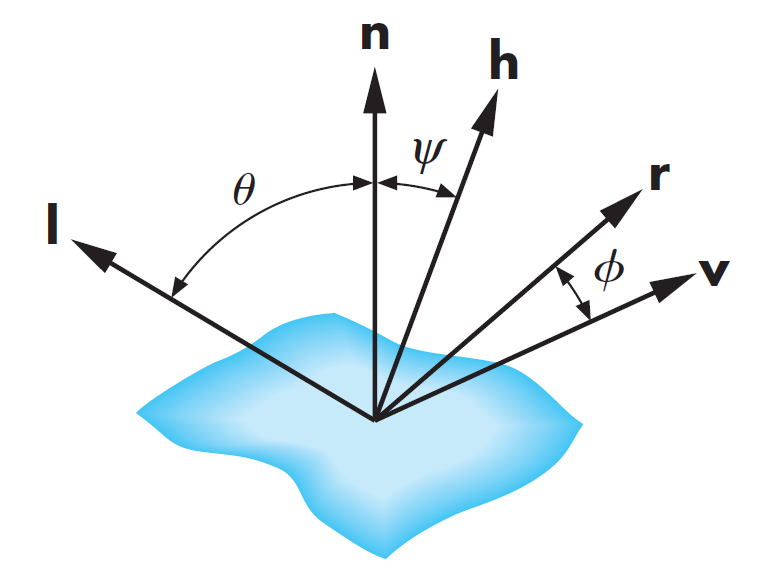
\includegraphics[scale=0.4]{./images/blinn-phong-reflection-model-vectors}\\
		\hline
		Sources& \cite{Comninos2005,Lengyel2003,shreiner2012} \\
		\hline
		Ref.\ By & \\
		\hline
	\end{tabular}
\end{minipage}\\

~\newline

\subsection{Output} \label{sec_Output}    
\begin{table}[h]
	\centering
	\begin{tabular}{|p{5cm}|p{10cm}|}
		\hline
		\textbf{Variability} & \textbf{Parameter of Variation} \\
		\hline
		Output file & Generated code file that when compiled renders a scene, 
		executable file that shows the rendered scene\\
		\hline
	\end{tabular}
	\caption{Parameters of Variation for Output.}
	\label{tbl:Output_Variations}
\end{table}

\section{Requirements}

This section provides the functional requirements, the business tasks that the
software is expected to complete, and the nonfunctional requirements, the
qualities that the software is expected to exhibit.

\subsection{Family of Functional Requirements}

\noindent \begin{itemize}

\item[R\refstepcounter{reqnum}\thereqnum \label{R_Inputs1}:] The library shall  
correctly read from file the input data for light source(s) and object(s).
\item[R\refstepcounter{reqnum}\thereqnum \label{R_Inputs2}:]The library shall 
verify that all input data meets constraints laid out in Table 
\ref{tbl:Input_Variations}.
\item[R\refstepcounter{reqnum}\thereqnum \label{R_Calculate1}:] The library 
shall correctly calculate the surface normals for object(s) based on shading 
model selected. 
\item[R\refstepcounter{reqnum}\thereqnum \label{R_Calculate2}:] The library 
shall calculate the incidence and reflection vectors off of object(s) 
surface(s) based on light position(s), object(s) properties, shading model and 
observer position.
\item[R\refstepcounter{reqnum}\thereqnum \label{R_Calculate3}:] The library 
shall calculate the light intensity based on light position(s), object(s) 
material properties, and shading model.
\item[R\refstepcounter{reqnum}\thereqnum \label{R_Calculate4}:] The library 
shall calculate the total luminance of object(s) faces based on light source 
type, light source position, object(s) material properties and position(s) and 
observer position.
\item[R\refstepcounter{reqnum}\thereqnum \label{R_Output}:] The library 
will output code for a lit and shaded scene.

\end{itemize}

\wss{I suggest changing the phrasing of the requirements to say the library
  offers these services.}

\subsection{Nonfunctional Requirements}

\noindent \begin{itemize}	
	\item[R\refstepcounter{reqnum}\thereqnum \label{NFR_Errors}:]System 
	responds with specific error message when user inputs contain errors (type 
	mismatch, data outside of constraints).
	\item[R\refstepcounter{reqnum}\thereqnum \label{NFR_Errors2}:]System 
	responds with specific error message when system cannot read input files.
	\item[R\refstepcounter{reqnum}\thereqnum \label{NFR_Default}:]System 
	provides a default setup for shading and reflection models.
	\item[R\refstepcounter{reqnum}\thereqnum \label{NFR_Default2}:]	System asks 
	user if they would like to use the default setup when shading and 
	reflection model information is missing from input.
	\item[R\refstepcounter{reqnum}\thereqnum \label{NFR_Usability}:]Users can 
	render a default scene (one cube, one point light in the centre of the 
	room, phong shading, and phong reflection model) faster than in OpenGL.
\end{itemize}

\wss{There is an issue on GitHub about the NFRs here mostly being FRs.}

\section{Likely Changes}    

\noindent \begin{itemize}

\item[LC\refstepcounter{lcnum}\thelcnum\label{LC_refraction}:] Refractive 
materials incorporated into family.
\item[LC\refstepcounter{lcnum}\thelcnum\label{LC_reflection_models}:] More 
reflection models incorporated into family.
\item[LC\refstepcounter{lcnum}\thelcnum\label{LC_normals}:] Variations on how 
normals are computed (e.g. partial derivatives) may be added to the family.

\end{itemize}

\section{Traceability Matrices and Graphs}
	\begin{table}
		\begin{tabular}{|l||l|l|l|l|l|l|l|l|l|l|l|}
			\hline
			& \aSref{as-geometrical_appx} & \aSref{as-illumination} & 
			\aSref{as-loc-vs-global} & \aSref{as-illum_constraint} & 
			\aSref{as-emission_constraint} & \aBref{as-coordinate_system} & 
			\aBref{as-coordinates} & \aBref{as-obsv_total} & 
			\aBref{as-object_representation} & 
			\aBref{as-object_representation2} & \aBref{as-object_refraction} \\
			\hline
			\tref{TM_Reflection} & X & & & & X & X & & & & & X \\
			\hline
			\dref{GD_diffReflect} & X & & X & & X & X & & & & & \\
			\hline
			\iref{IM_LamDiffuse} &X&X&X&X&X& & & & & &\\
			\hline
			\iref{IM_HalfLam} &X&X&X&X&X& & & & & & \\
			\hline
			\iref{IM_Phong} & X&X&X&X&X& &X&X& & & \\
			\hline
			\iref{IM_Blinn_Phong}& X&X&X&X&X& &X&X& & & \\
			\hline
			\ddref{DD_Dot_Product} & & & & & &X&X& & & & \\ 
			\hline
			\ddref{DD_Cross_Product} & & & & &&X&X& & & & \\		
			\hline
			\ddref{DD_Intensity_ambient} &X&X&X&X& & & & & & & \\
			\hline
			\ddref{DD_Intensity_diffuse} & &X& & &X& & & & & &X\\
			\hline
			\ddref{DD_Intensity_specular}& &X& & &X& & & & & &X\\			
			\hline
			\ddref{DD_Intensity_Total} & &X&X&X&X& & & & & &X\\		
			\hline
			\ddref{DD_Intensity_PointSource_Distance} &X&X& & & &X&X& & & & \\
			\hline
			\ddref{DD_Flat_Shading} &X& && &X&X&X& &X& & \\
			\hline
			\ddref{DD_Gouraud_Shading} &X&X&X&&X&X&X& &X&X&X\\			
			\hline
			\ddref{DD_Phong_Shading} &X&X&X&&X&X&X& &X&X&X\\			
			\hline
			\lcref{LC_normals} &X& & & & &X&X& &X&X& \\			
			\hline
			\lcref{LC_reflection_models} & &X&X&X&X& &X& & & 
			&X\\						
			\hline
			\lcref{LC_refraction} & &X&X&X&X& & & & & &X\\
			\hline						
		\end{tabular}
		\caption{Traceability Matrix matching Scope and Build Time Assumptions 
		to Theoretical Models, General Definitions, Instance Models, Data 
		Definitions and Likely Changes.}
	\end{table}	

\section{Appendix}

\subsection{First Stage of Implementation}
\plt{In this section specify the family member, or sub-family, that you will be
	implementing for CAS 741.  You should specify the value for all of your
	variabilities, along with the binding time.  A tabular representation will
	probably be the easiest way to convey this information.}

In this project we will be implementing all of the family members touched by 
the orange line in Figure \ref{fig:prob-domain-analysis}.

\wss{I think we need more information than this.  What are the values of the
  variabilities in your table?  For instance, what objects are you allowing?}


\newpage

\bibliographystyle {plainnat}
\bibliography {../refs/References}

\newpage

\end{document}